%\documentclass{recpad2k}
\documentclass[extendedabs]{recpad2k}

\usepackage{enumitem}
\usepackage{graphicx}

\title{Assignment 2: The Raven Test \\ \LARGE{In Search for Group Differences}}

% Enter the paper's authors in order
% \addauthor{Name}{email/homepage}{INSTITUTION_CODE}
\addauthor{Filipe Pires}{85122}{1}
\addauthor{João Alegria}{85048}{1}
\addauthor{Ana Tomé}{ana@ua.pt}{12}

% Enter the institutions
% \addinstitution{Name\\Address}
\addinstitution{
   Department of Electronics, Telecommunications and Informatics,\\
   University of Aveiro, Portugal
}
\addinstitution{
   Institute of Electronics and Informatics Engineering of Aveiro,\\
   University of Aveiro, Portugal
}

% Any macro definitions you would like to include
% These are not defined in the style file, because they don't begin
% with \bmva, so they might conflict with the user's own macros.
% The \bmvaOneDot macro adds a full stop unless there is one in the
% text already.
\def\eg{\emph{e.g}\bmvaOneDot} 
\def\Eg{\emph{E.g}\bmvaOneDot}
\def\etal{\emph{et al}\bmvaOneDot}

%------------------------------------------------------------------------- 
% Document starts here
\begin{document}

\maketitle

\begin{abstract}
   \vspace{-10pt}
   {\bf 
      The search for trustworthy methodologies of determining a measurable intelligence index has been a quest of our brightest minds for decades.
      Raven matrices tests have proved to have widespread practical use as a measure of intelligence.
      They are a source of data for many studies on the general population as they seem promising tools for contexts such as psychometric tests or clinical assessment.

      In one study on the application of these matrices to groups of students from different backgrounds, questions emerged regarding the possibility of clear 
      differences between Multimedia and Informatics students.
      In this paper we present the statistical analysis applied to the tests results with the help of ML classification techniques in search for determining 
      whether any of the two groups showed significant advantages over the other.
   }
\end{abstract} 

% \begin{abstract}
% This document demonstrates the format requirements for papers submitted
% to the Portuguese Conference on Pattern Recognition.  The format is designed for
% easy on-screen reading, and to print well at one or two pages per sheet.
% Additional features include: pop-up annotations for
% citations~\cite{Authors06,Mermin89}; a margin ruler for reviewing; and a
% greatly simplified way of entering multiple authors and institutions.

% {\bf All authors are encouraged to read this document}, even if you have
% written many papers before.  As well as a description of the format, the
% document contains many instructions relating to formatting problems and
% errors that are common even in the work of authors who {\em have}
% written many papers before.
% \end{abstract}

%------------------------------------------------------------------------- 

\section{Introduction}

Raven's Advanced Progressive Matrices (RAPM) is a non-verbal group test typically present in educational or clinical settings, as it is used in measuring 
abstract reasoning and regarded as an estimate of fluid intelligence \cite{rapm}.
Examples of related test are Naglieri Nonverbal Ability or Spacial Ability Tests.
Their practical use is very extended, and applicable to both adults and children.
Nevertheless, studies that resort to them usually focus on populations containing groups with specific differences in order to draw conclusions from these differences.
Examples of these studies are on different military sections, or different mental disabilities.

In the study whose collected data was used for our analysis \cite{study}, the aim was to compare students from different fields in terms of learning styles effectiveness.
Several tests such as Kolb and VAK or Hermann dominances allow to distinguish some learning styles like: Accommodator, Assimilator, Auditory, Convergent,
Divergent, Kinesthetic and Visual.
But beyond this, the researchers also applied the RAPM tests to reach more robust conclusions, and combine all results in a meaningful way.
In this paper we focus only on the data related to the second set of tests.

The population that performed the Raven tests was a group of 45 university students, 21 of Design and Multimedia and 24 of Informatics Engineering.
48 problems were presented to both populations, divided into 2 phases: during the first 12, the participant would receive a feedback about his/her answer; 
for the remaining 36 no feedback was given.
During test execution, electroencephalographic (EEG) signals were registered while participants performed the tasks, using Enobio 8 EEG recording headset and 8 
channels: \textit{F3, F4, T7, C3, Cz, C4, T8} and \textit{Pz}.

Our aim was to determine from this estimated measurement of intelligence whether both groups hold characteristics significantly different from each other by 
building classification algorithms that interpret the EEG signals and other time-related metrics as features and attempt to predict which class of students a 
new entry belongs to.
We also intended to compare our conclusions with those obtained by the original researchers.

% \section{Introduction}
% \label{sec:intro}
% The proceedings of RecPad (the Portuguese Conference on Pattern Recognition) will be published only in electronic form.  This document
% illustrates the required paper format, and includes guidelines on
% preparation of submissions.  Papers which fail to adhere to these
% requirements may be rejected at any stage in the review process.

% \LaTeX\ users should use this template in order to prepare their paper.
% Users of other packages should emulate the style and layout of this
% example.  Note that best results will be achieved using {\tt pdflatex},
% which is available in most modern distributions.

% \subsection{Paper length: two pages including bibliography and title}
% Papers must be 2~pages in length, {\em including} the bibliography.  Length
% is counted from the bottom of the title on the first page.  Therefore, the
% bibliography should begin eight lines into page ten.  This is an
% approximate measure, intended to encourage brevity, but authors should keep
% in mind that blatant disregard of this instruction will cause reviewers to
% require greater originality and impact of the submission.  {\bf Papers which are
% clearly overlength will not be reviewed}.  This includes papers where the
% margins and formatting are deemed to have been significantly altered from
% those laid down by this style guide.  The reason such papers will not be
% reviewed is that there is no provision for supervised revisions of
% manuscripts.  The reviewing process cannot determine the suitability of the
% paper for presentation in nine pages if it is reviewed in twelve.

\section{Dataset \& Feature Extraction}

The dataset provided for this assignment had data both related to individual participants and aggregations with averages.
For our intentions, we were interested only in the individual results, so we used the data from the "Trial" folder, containing 4 XML spreadsheets: two for the 
Informatics students (referred to as DEI), two for the Multimedia students (referred to as ESEC).
Departments were split as one file contains the right answers of the students on the Raven tests and the other contains the wrong answers.

Each file contains information about 36 task executions, with an entry for each student and a column for each metric. 
The relevant marks for the signal analysis are around: 
\begin{itemize}[noitemsep,nolistsep]
\item Problem Display
\item Possible Solutions Display
\item Student's Answer
\end{itemize}
\vspace{2pt}
On the problem and possible solutions displays, the considered signal processing windows were [-75 500] ms.
On the student's answer, the window was [-500 500] ms.

Some of the considered metrics were:
\begin{itemize}[noitemsep,nolistsep]
\item Peak \& Latency for P100 PZ, P100 CZ, P300 CZ signals
\item F3, F4 Stress signals
\end{itemize}
\vspace{2pt}
P100 and P300 were chosen because of attentional and relationship characteristics that have sometimes been attributed to them.
They are defined in the first time interval and their latency and amplitudes are stored, considering only the relevant channels.
This data was used as time features for the classification algorithms.

For the frequency features, the energy of the characteristic bands is estimated in all defined windows.
This Engergy (E) is then used to compute other higher level features called energy ratios, considering several signal channels:
\begin{itemize}[noitemsep,nolistsep]
\item Stress Index
\item Mental Fatigue
\item Alpha Lateralization
\item Immersion Index
\end{itemize}
\vspace{2pt}
All of these features are present in the dataset spreadsheets.

As in any classification challenge, we needed to divide the data into training and testing entries.
The way we divided the results was 80\% for the training of the classifiers and 20\% for testing, due to the relatively reduced size of the dataset.

% The bibliography should begin immediately after the paper text.  It may
% be of any length, within reason.  It should {\em not} include
% annotations, figures, or any other paraphernalia intended to subvert the
% paper length requirement.

% \begin{figure*}
% \begin{tabular}{ccc}
% \bmvaHangBox{\fbox{\parbox{2.7cm}{~\\[2.8mm]
% \rule{0pt}{1ex}\hspace{2.24mm}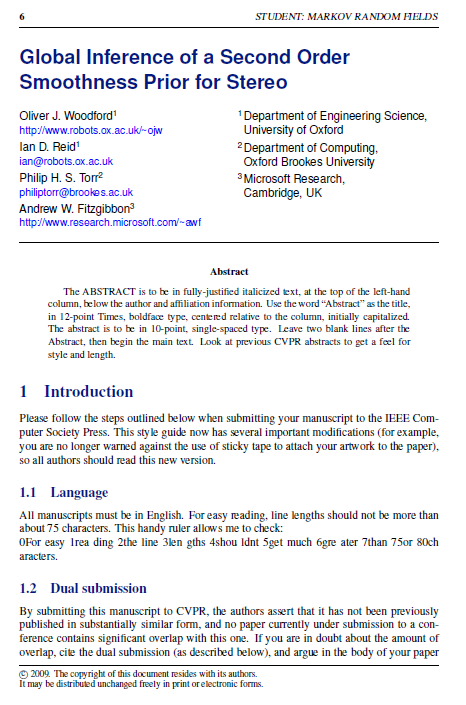
\includegraphics[width=2.33cm]{images/eg1_largeprint.png}\\[-0.1pt]}}}&
% \bmvaHangBox{\fbox{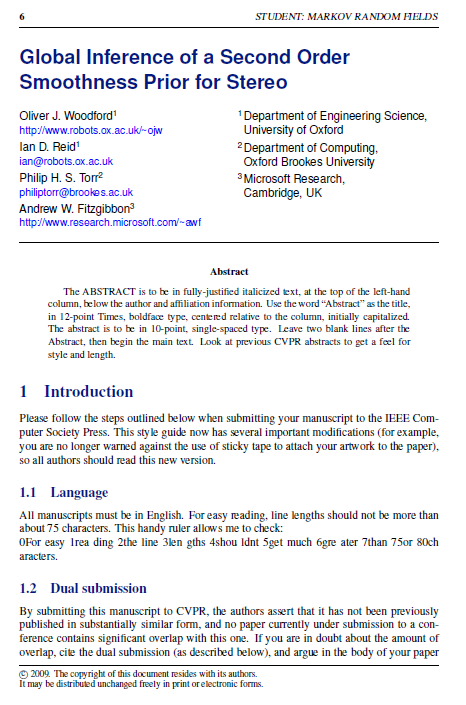
\includegraphics[width=2.8cm]{images/eg1_largeprint.png}}}&
% \bmvaHangBox{\fbox{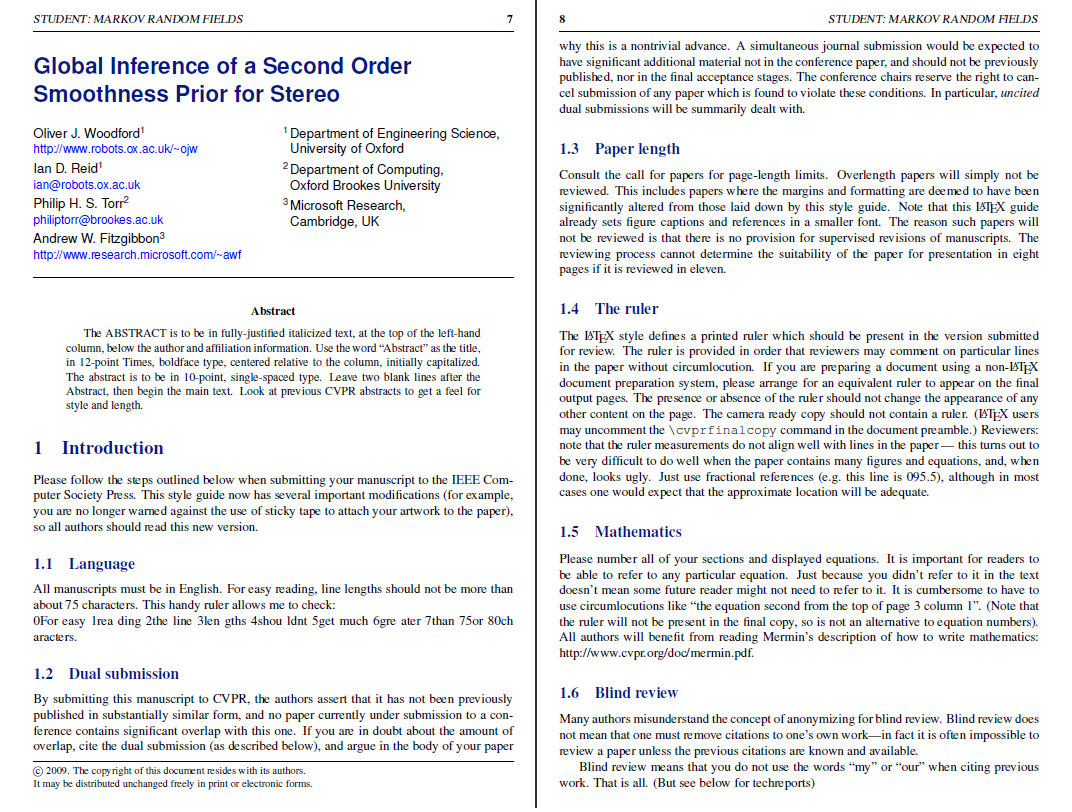
\includegraphics[width=5.6cm]{images/eg1_2up.png}}}\\
% (a)&(b)&(c)
% \end{tabular}
% \caption{It is often a good idea for the first figure to attempt to
% encapsulate the article, complementing the abstract.  This figure illustrates
% the various print and on-screen layouts for which this paper format has
% been optimized: (a) traditional print format; (b) on-screen
% single-column format, or large-print paper; (c) full-screen two column, or
% 2-up printing. }
% \label{fig:teaser}
% \end{figure*}



% \subsection{Citations}
% When citing a multi-author paper, you may save space by using ``{\em et
% alia}'', shortened to ``\etal'' (not ``{\em et.\ al.}'' as ``{\em et}'' is
% a complete word.)  The provided \verb'\etal' macro is a useful {\em aide
% memoire} in this regard.  However, use it only when there are three or more
% authors.  Thus, the following is correct: `` Frobnication has been trendy
% lately.  It was introduced by Alpher~\cite{Alpher02}, and subsequently
% developed by Alpher and Fotheringham-Smythe~\cite{Alpher03}, and Alpher
% \etal~\cite{Alpher04}.''

% This is incorrect: ``... subsequently developed by Alpher \etal~\cite{Alpher03} ...''
% because reference~\cite{Alpher03} has just two authors.  If you use the
% \verb'\etal' macro, then you need not worry about double periods
% when used at the end of a sentence as in Alpher \etal.

%For this citation style, keep multiple citations in numerical (not
%chronological) order, so prefer

% We use {\tt natbib}, so citations in random order are nicely sorted:
%  \cite{Alpher03,Alpher02,Authors06b,Authors06}.  However, we don't use the
% compress option, as we want each reference to have its own hyperlink and
% popup window.

%------------------------------------------------------------------------- 
% \subsection{Footnotes}

% Please use footnotes\footnote {This is what a footnote looks like.  It
% often distracts the reader from the main flow of the argument.} sparingly.
% Indeed, try to avoid footnotes altogether and include necessary peripheral
% observations in 
% the text (within parentheses, if you prefer, as in this sentence).  If you
% wish to use a footnote, place it at the bottom of the column on the page on
% which it is referenced. Use Times 8-point type, single-spaced.


% \begin{figure*}
% \begin{center}
% \fbox{\rule{0pt}{2in} \rule{.9\linewidth}{0pt}}
% \end{center}
%    \caption{Example of a short caption, which should be centered.}
% \label{fig:short}
% \end{figure*}

%------------------------------------------------------------------------- 
% \subsection{The ruler}
% The \LaTeX\ style defines a printed ruler which should be present in the
% version submitted for review.  The ruler is provided in order that
% reviewers may comment on particular lines in the paper without
% circumlocution.  If you are preparing a document using a non-\LaTeX\
% document preparation system, please arrange for an equivalent ruler to
% appear on the final output pages.  The presence or absence of the ruler
% should not change the appearance of any other content on the page.  The
% camera ready copy should not contain a ruler. (\LaTeX\ users may remove
% the \verb'[review]' option from the \verb'\documentclass' statement.)
% Reviewers: note that the ruler measurements do not align well with lines
% in the paper --- this turns out to be very difficult to do well when the
% paper contains many figures and equations, and, when done, looks ugly.
% Just use fractional references (e.g.\ this line is $210.5$), although in
% most cases one would expect that the approximate location ($210$ in the
% previous example) will be adequate.


\section{Data Quality \& Normalization}\label{data}

The first thing we did with the raw data was to correlate every possible pair of features through 2-Dimensional projections.
This would help us understand how was the data distributed in the multidimensional space and whether there were clear separations between the two classes 
(DEI and ESEC).
Table \ref{fig:feature} is the visual representation of this correlation as an organized collection of:
\begin{itemize}[noitemsep,nolistsep]
\item Histograms - presented in the diagonal composed by the feature related with itself and describing the value distribution inside that given feature.
\item Scatter Plots - presented in all other entries and describing the value distribution between feature pairs.
\end{itemize}

Through the analysis of this table, we can gather some important conclusions. 
The most clear characteristic detected was the presence of outliers, one that was already expected and needed to be taken care of.
The second was the fact that the data in all pairs of features doesn't appear to be separable, i.e. there should be something resembling two groups, one for 
each class, or point clouds in some of the projections.
If this was visible, the possibility of actually existing a difference between groups would be likelier to be true.
However, that does not seem to be the case, since in most cases we are presented with uniform distributions, gaussian distributions or simply the grouping of 
all data in a unique central point. 
It is important to mention that this does not automatically mean that a solution could not be found, as the group distinction we were looking for could depend 
on more than two variables and so could indeed not be visible in the 2-Dimensional projections.

Once familiarized with the data, we proceeded to pre-processing it so that the models we intended to to apply would have the best chances of finding the 
distinguishing factors.
To do this, we centered the data and removed the detected outliers.
Equation \ref{zscore} contains the formula of the \textit{Z-Score} algorithm applied to each feature to center all values.
Then, we removed any data entry that contained a \textit{Null} value, since that would cause problems for the models' processing.
Finally we removed the still existing outliers with the help of equation \ref{outliers}, that ensures that entries with very distant values from the standard 
deviation are not considered as they do not have valuable information to offer.

\begin{equation}\label{zscore}
   z_{i} = \frac{x_{i} - \mu}{\delta}
\end{equation}

\begin{equation}\label{outliers}
   |x_{i}-\mu| < 3\times\delta
\end{equation}

\section{Classifiers}\label{classifiers}
In this section we will present and give a brief summary of all the machine learning models used in this study. We chose this models since through a brief state 
f the art analysis we concluded that these are the most common and suggested models when handling machine learning problems, and also the ones that achieve the 
best performance overall. We also found that some of the models used are to most recommended when handling with data similar to our context.

\subsection{Support Vector Machine}
\textit{Support Vector Machine}, commonly denoted as SVM, is a supervised machine learning model that with the supplied training set, maps the different data 
entries into a multidimensional space in a way that the widest possible gap exists between the data of each class. Based in that gap a model is created and a 
decision rule defined that when feed new data tries to assign a class to that entry by comparing against the decision rule already mentioned.

The most common and simple SVM application tries to creates a linear division between the presented classes. Another alternative that allows more complex 
decision rules is the application of a kernel trick, that implicitly maps tha data to a higher-dimensioned feature space which may enable a better separation 
of the data.

\subsection{MultiLayer Perceptron}
\textit{MultiLayer Perceptron} is a class of feedforward artificial neural network is another supervised machine learning model. MLP is sometimes strictly 
refers to networks composed of multiple layers of perceptrons. Perceptron is also a supervised learning algorithm capable of doing binary classifications 
according to a linear predictor function. The power of the MLP is the junction of several of those perceptrons that individually don't have the a good 
performance, but the combine performance can reach significant values.

This junction normally follows a standard architecture divided in layers, firstly a input layer, followed by one or more hidden layers and an output layer. 
The input and the output layers are the ones that interact with the exterior, being the first, as the name indicates teh one where the data should be injected 
at and the second where the result will be presented. The hidden layers is where the main learning occurs and where the most amount of fine-tunning is applied. 
In this entire architecture the number of layers and the number of neurons(singular cell inside a layer) can be tunning to improve the model performance.

\subsection{Decision Tree}
This supervised learning algorithm, as the name suggests, uses a tree like structure to support the data classification decision and aims to convert the 
observed patterns in the train data into conclusions about the data classes. The construction of this auxiliary structure is quite simple and straightforward, 
consisting in assigning a condition to each new branch, causing that the structure will converge in having only one class in leaf nodes, defining the conditions 
required to identify the existing classes. These condition choices must be taken with caution since a poor decision in this phase may cause a drastic decrease 
in the performance of the overall model. Many times this process uses \textit{Entropy} as a guide, where \textit{Entropy} indicates, in a very high level 
approximation, the level of confusion/chaos/randomness of a set of information, thereby if the data tested belongs to only one class, the entropy should be 0 
and the system knows that that data portion doesn't need to be divided anymore.

\subsection{Random Forest}
Similarly to the last model, \textit{Random Forest} is also a supervised learning model and also uses tree structures to support the models' classification 
decisions. The difference is that in this approach the model uses several instances of Decision Trees, with the purpose of since sometimes Decision Tree don't 
generate the best performance possible, using multiple and dividing the problem so that not every tree specializes in all the features, dividing and conquering 
the problem.

\subsection{K Nearest Neighbors}
The last model that we decided to test was the \textit{K Nearest Neighbors}, which although being one of the simplest learning algorithms, still is essential 
in the Machine Learning area. Still in the supervised learning algorithm area, this model uses a very simple approach to it's classification process; by 
representing every train data entry in a multidimensional space, once presented with new data, the model simple represents that new entry in the mentioned 
multidimensional space and verifies the class of the K nearest points(train entries), and the most frequent class in that K dataset is the one that is assigned 
to that new data entry. 


\section{Models Fine Tuning}\label{parameters}

\subsection{Performance Evaluation}

Once the classification models were implemented, we needed to measure their performance.
This was accomplished through the confusion matrix, a matrix that correlates a model's predictions with the true values and gives us the number of: 
true positives (TP) and true negatives (TN), the correct predictions of wether an entry belongs to 1 of the classes or not; false positives (FP) and 
false negatives (FN), the incorrect predictions.
The class defined as true can be any of the two, as the process is equivalent when inversed.
In our case this was something done internally to the tools used, beyond our reach.

With these values, we were able to compute 4 widely used performance metrics:
\begin{itemize}[noitemsep,nolistsep]
\item Accuracy, given by $A = \frac{TP + TN}{TP + TN + FP + FN}$
\vspace{3pt}
\item Precision, given by $P = \frac{TP}{TP + FP}$
\vspace{3pt}
\item Recall, given by $R = \frac{TP}{TP + FN}$
\vspace{3pt}
\item F1-Score, given by $F = \frac{2 \times P \times R}{P + R}$
\vspace{3pt}
\end{itemize}
During our analysis we only consider \textit{A} and \textit{F}, as accuracy alone is not enough to evaluate the models (not robust to several aspects) and F1 
correlates precision and recall very effectively.

\subsection{Parameters Variation}

In this section we present the manipulation of the hyperparameters related to each of the implemented algorithms, in search for better performances.

For the SVM, using the default parameters with the Radial Basis Function (RBF) kernel, the accuracy was around 55\%.
The sigmoid kernel proved to be more appropriate for the dataset as it increased both the accuracy to 57\% and the F1-Score from 68\% to about 73\%.
The remaining parameters such as the kernel coefficient (altered between "auto" and "scale"), tolerance for stopping criterion (ranged from $1.0 \times 10^{-3}$
to $0.1$), decision function shape or maximum number of iterations proved to have no significant effect when carefully altered.

Moving on to MLP, the default parameters of the neural network were the following:
"relu" activation layer, "adam" solver for weight optimization, L2 penalty and tolerance both at $1.0 \times 10^{-4}$, "constant" learning rate and an 
architecturewith 3 hidden layers of 13 nodes.
This configuration resulted in an accuracy of 54\%.
The best found configuration turned out to be the following: "identity" activation layer (although not very different from the original), "lbfgs" solver (that 
proved to be more effective than "adam" for our dataset), a simples architecture with only 2 hidden layers of 10 and 5 nodes (that had the same effect as the 
more complex one), and the remaining parameters with the default values (as changing them only reduced at least one of the performance metrics).
The final performance was of 56\% of accuracy and 67\% of F1-Score.

The DTs showed worse results in all metrics.
Changing the criterion (function to measure the quality of a split) from "gini" to "entropy" showed no improvements, nor did tweaking the trees' maximum depth 
or minimum number of samples required to split an internal node.
Defining the weights associated with classes made precision fall 2 percentiles.
The best accuracy found was 53\% with F1 at 58\%.
The addition of Random Forests was an attempt to improve these values, as RFs use several DTs to return a combined answer theoretically better than one 
considering only one DT.
However, from our studies, Random Forests were only able to improve F1-Score, and only slightly with a maximum value of 60\%.

Finally we dedicated our attention to KNN.
Reducing the number of K nearest neighbors from 5 to 3 seemed to have a considerably good effect on its performance, raising 2\% of the model's accuracy.
Also, defining the algorithm used for computing the nearest neighbors was futile, as all alternatives had no effect whatsoever.
Altering the distance calculation formula from euclidean to any other reduced the precision slightly.
The best configuration gave an accuracy of 53\%, with F1 at 60\%.

\subsection{Feature Manipulation}

Lorem ipsum ...


\section{Results Discussion}
After executing all the parameter variation study, the feature analysis as well as some feature addition in hopes of adding some extra meaningful information 
to the already existing data, the best performance results were the ones presented in Section \ref{parameters}.
Although not the most satisfying results, since when conducting a machine learning problem the aim is to obtain a model with a defined set of hyperparameters 
that generate a good performance with good values(close to 100\%) on its performance indicators, but the results obtained in this study have a reason to be.

Referring to Section \ref{data}, one of the conclusions taken from analyzing the Figure \ref{fig:feature} was that no obvious division was observable in the 
data projections in the different feature pair plane. Although this conclusion not absolute proof that the data isn't separable, the results of the tested 
model indicate that that is the case. This can be caused by several reasons, ranging from the dataset quality, the models used, the tunning of the 
hyperparameters or even the case of overfitting of the training data. 

Through a deeper analysis over the data itself we didn't found any aspect that could compromise our study; the origin of the data and the metrics gathered 
seemed to be the most adequate for this type of study; the features also seemed to be widespread enough to encapsule all the possible signals related to this 
study, such as fatigue, immersion, stress, \dots. In relation to the models used, as already mentioned in Section \ref{classifiers} are state-of-the-art, 
therefor should perform well enough with the dataset presented, and for that matter, with any dataset. The parameters variation was probably the portion of 
the report study that took the longer, since we made a meticulous study of the parameters for all the models trained as detailed in Section \ref{parameters}. 
For that reason we can conclude that the parameter choice is also not the problem. Finally, in relation to the overfitting problem, the fact that all the models 
used gave similar results, it's quite improbable that all of them suffer from the overfitting. That allows us to also remove this problem from our list of 
possible issues.

Knowing that the variables in our reach are properly tested and in theory are correct, we can only conclude that the data itself is inseparable. 
This means that the two classes presented, the students from \textit{DEI} and the students from \textit{ESEC}, although obviously two different groups in this 
study, the conducted experiment indicates that in terms of the \textit{RAVEN} intelligence estimation test there is no difference between the two groups.

Finally, in spite of all models produced a similar performance, where the \textit{Accuracy} averaged in the 55\% mark and the \textit{F-Score} averaged in the 
65\% mark. This difference is due to the fact that both \textit{Precision} and \textit{Recall} are slightly higher than the \textit{Accuracy}, which indicates 
that however the classification is almost random, in reality the models are able to generate more true results than negative results, which is quite interesting 
given the limitations observed from the models.

\section{Conclusions \& Future Work}

Determining differences between populations is not a trivial task.
The subjectiveness element of intelligence measurements increase the complexity of such problem, and so clear conclusions are very hard to find.
Nevertheless there are many cases where, when the correct analysis tools are applied, solid conclusions are reached - even if they are precisely that 
no conclusion can be drawn - and this is exactly that case.

By discussing our results and the similarity of outcomes between very different classification models, and comparing our results with those obtained in the 
original study conducted by the dataset authors, we were able to understand that in fact there are no significant differences between Multimedia and Informatics 
students in terms of intelligence.
In fact, this is parallel to our initial suppositions, as both classes require highly cognitive skills and problem solving capacities, even though applied to 
very different situations.

For future work, we believe it would not be a good idea to attempt implementing other classification algorithms, as they would very much likely return similar results.
Instead, if the interest of analyzing the same dataset remained, we would probably address different questions such as "Are there any differences between 
women and men within these courses?", or "Is it possible to predict whether a student will get the answer right to one of the Raven's tasks or not?".

Our overall perspective on the project is very positive, even though we, as Informatics students, were wishing to find advantages on the side of the 
students with a similar background as ourselves.
Nevertheless, we found the use of Jupyter Notebooks very practical and adequate to assignments such as this and, as it allowed us to segment the work to be done,
we were able to keep a good balance and work distribution between group elements throughout the development.


% \begin{table}
% \begin{center}
% \begin{tabular}{|l|c|}
% \hline
% Method & Frobnability \\
% \hline\hline
% Theirs & Frumpy \\
% Yours & Frobbly \\
% Ours & Makes one's heart Frob\\
% \hline
% \end{tabular}
% \end{center}
% \caption{Results.   Ours is better.}
% \end{table}

% \subsection{Mathematics}

% Please number all of your sections and displayed equations.  It is
% important for readers to be able to refer to any particular equation.  Just
% because you didn't refer to it in the text doesn't mean some future reader
% might not need to refer to it.  It is cumbersome to have to use
% circumlocutions like ``the equation second from the top of page 3 column
% 1''.  (Note that the ruler will not be present in the final copy, so is not
% an alternative to equation numbers).  All authors will benefit from reading
% Mermin's description~\cite{Mermin89} of how to write mathematics.


%------------------------------------------------------------------------- 

\begin{thebibliography}{00}
\bibitem{rapm} Warren B. Bilker et al., "Development of Abbreviated Nine-item Forms of the Raven’s Standard Progressive Matrices Test", \url{https://www.ncbi.nlm.nih.gov/pmc/articles/PMC4410094}, accessed in December 2019.
\bibitem{study} Felisa M. Córdova et al., "Identifying Problem Solving Strategies for Learning Styles in Engineering Students Subjected to Intelligence Test and EEG Monitoring", \url{https://www.sciencedirect.com/science/article/pii/S1877050915014787}, Procedia Computer Science 55 (2015), accessed in December 2019.
\bibitem{assign2} A. Tomé, "Data Mining Assignment", \url{https://elearning.ua.pt/pluginfile.php/1496406/mod_resource/content/3/ED_HCT_Raven.pdf}, accessed in December 2019.

\end{thebibliography}
% https://en.wikipedia.org/wiki/Support-vector_machine
% https://en.wikipedia.org/wiki/Multilayer_perceptron
% https://en.wikipedia.org/wiki/Perceptron
% https://en.wikipedia.org/wiki/Decision_tree
% https://en.wikipedia.org/wiki/K-nearest_neighbors_algorithm

% \section{References}

% List and number all bibliographical references in 9-point Times,
% single-spaced, at the end of your paper. When referenced in the text,
% enclose the citation number in square brackets, for
% example~\cite{Authors06}.  Where appropriate, include the name(s) of
% editors of referenced books.

\appendix
\begin{figure}[h]
    \centering
    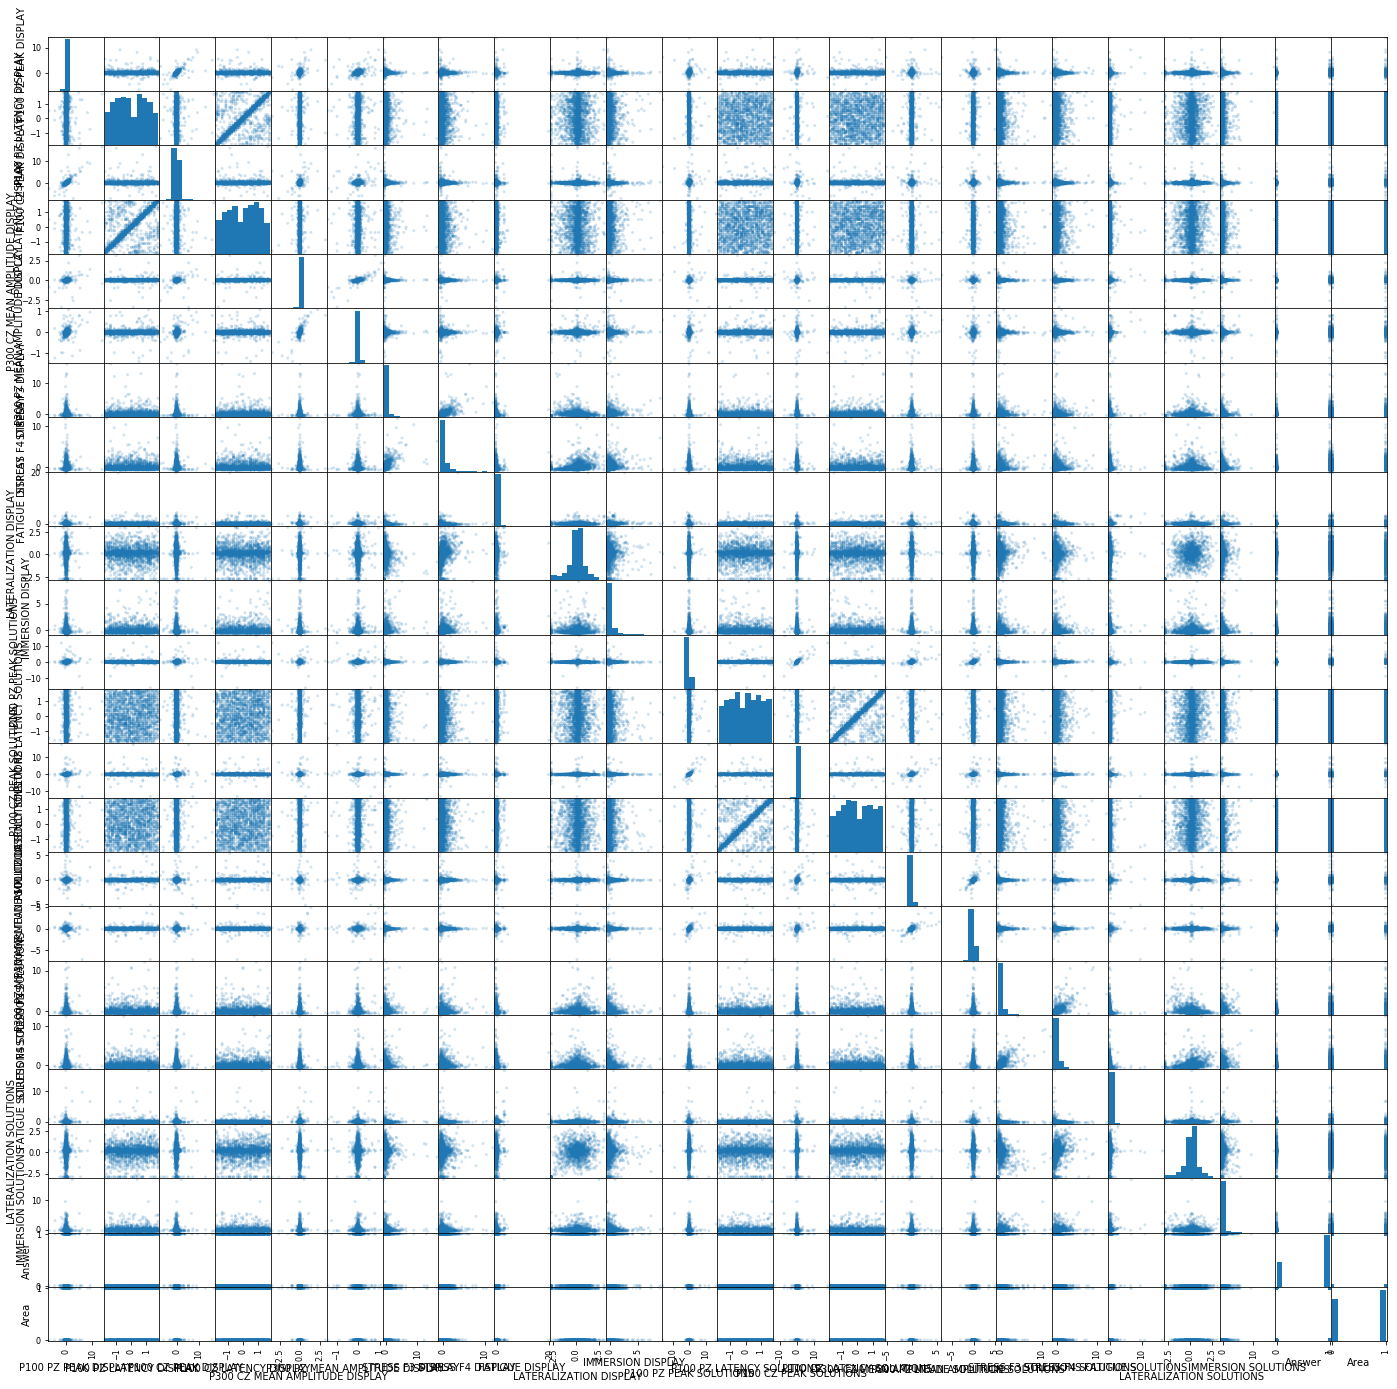
\includegraphics[width=2\linewidth]{featurecorrelation.png}
    \caption{Feature Correlations}
    \label{fig:feature}
\end{figure}


% %------------------------------------------------------------------------
% \section{Color} 

% Color is valuable, and will be visible to readers of the electronic copy.
% However ensure that, when printed on a monochrome printer, no important
% information is lost by the conversion to grayscale.

% \bibliography{recpad_review}

\end{document}
